\section{Deep Gated Network and Deep Gated Network Without Activations}\label{sec:dgn-no-act}
In this section, we make a brief presentation of the preliminaries dual view formulation for a fully connected (FC) DNN with ReLUs in \citep{npk}. We consider a FC-DNN with `$d$' layers and  $w$  hidden units in each layer. The quantites `path feature' and `path value' in \Cref{sec:intro} will henceforth be called as \emph{neural path feature}(NPF) and \emph{neural path value} (NPV); these are defined in \Cref{def:npf-npv}. \Cref{prop:npf-npv} show that the output is the inner product of the NPF and NPV. \Cref{lm:npk} shows the relationship between the \emph{neural path kernel} (NPK), the Gram matrix of the NPFs, and a correlation matrix capturing subnetwork overlaps. 

\begin{definition}\label{def:npf-npv}
A path starts from an input node, passes through a weight and a hidden unit in each layer and ends at the output node. We define the following quantities for a path $p$:
\emph{
\begin{tabular}{lcl}
 Activity&:& $A_{\Theta}(x,p)$ is the product of the `$d-1$' gates in the path. \\
Value&:& $v_{\Theta}(p)$ is the product of the `$d$' weights in the path.\\
Feature&:&   $\phi_{\Theta}(x,p)$ is the product of the signal at the input node of the path and $A_{\Theta}(x,p)$.\\
\end{tabular}
}

The \emph{neural path feature} (NPF) given by $\phi_{\Theta}(x)=\left(\phi_{\Theta}(x,p),p=1,\ldots, \Pfc\right),\in\R^{\Pfc}$ and the \emph{neural path value} (NPV) given by $v_{\Theta}=\left(v_{\Theta}(p),p=1,\ldots,\Pfc\right),\in\R^{\Pfc}$.
\end{definition}

\begin{proposition}\label{prop:npf-npv}
The output of the DNN is then the inner product of the NPF and NPV: 
\begin{align}\label{eq:inner}
\hat{y}_{\Theta}(x)=\ip{\phi_{\Theta}(x),v_{\Theta}}=\sum_{p\in[P]}  \phi_{\Theta}(x,p) v_{\Theta}(p)
\end{align}
\end{proposition}
\begin{figure}[t]
\centering
\resizebox{0.9\columnwidth}{!}{
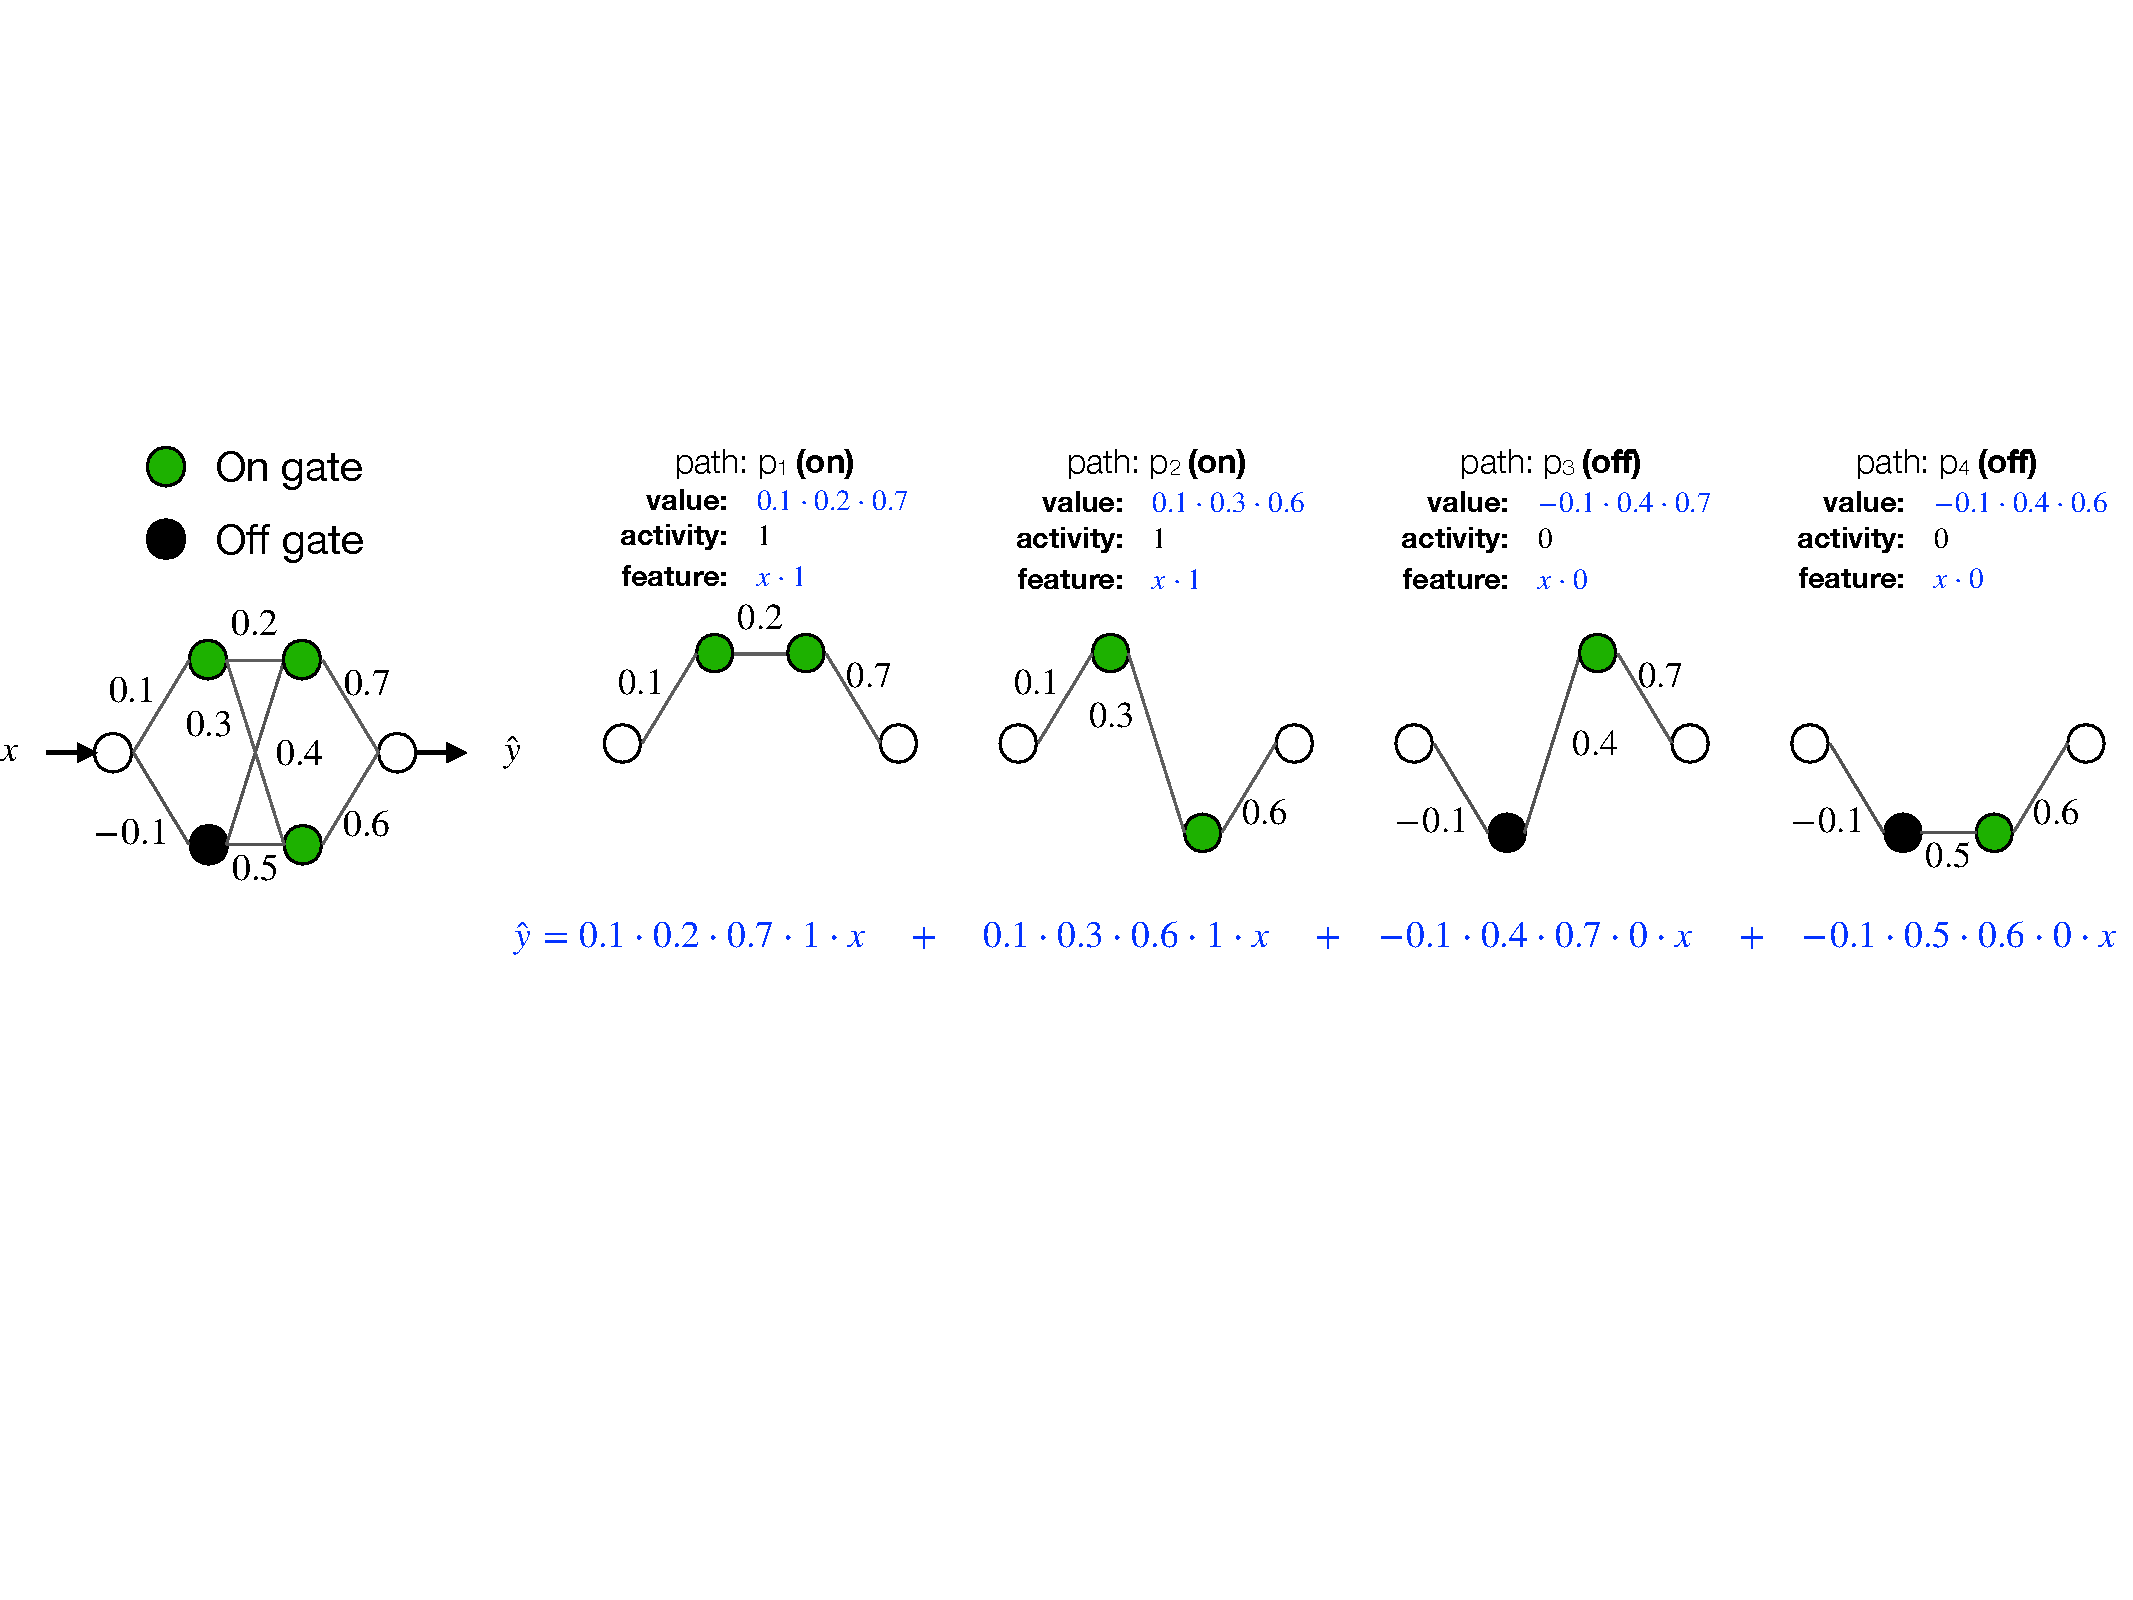
\includegraphics[scale=0.5]{figs/paths.pdf}
}
\caption{Illustration of \Cref{def:npf-npv} and \Cref{prop:npf-npv} in a  toy network with $2$ layers, $2$ gates per layer and $4$ paths. Paths $p_1$ and $p_2$ are `on' and paths $p_3$ and $p_4$ are `off'. The value, activity and feature of the individual paths are shown. $\hat{y}$ is the summation of the individual path contributions.}
\label{fig:paths}
\end{figure}

\begin{figure}
\centering
\begin{minipage}{0.8\columnwidth}
\begin{minipage}{0.49\columnwidth}
\resizebox{0.99\columnwidth}{!}{
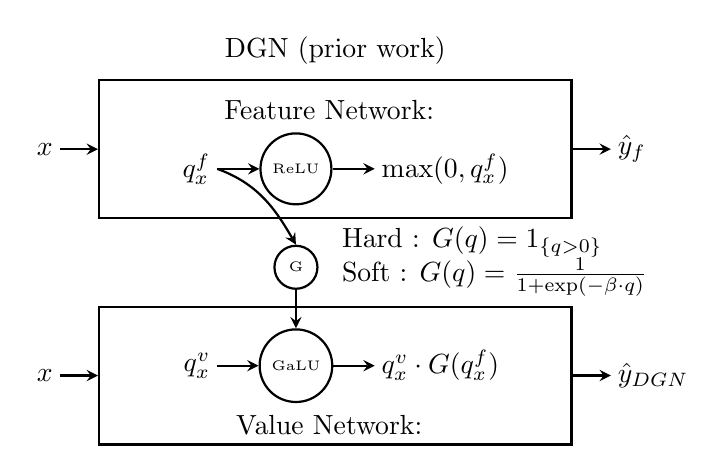
\begin{tikzpicture}

\node []  (fntext)at (3.5,1.5) {DGN (prior work)};
%Feature Network
\node [draw,
	minimum width=6cm,
	minimum height=1.75cm,
	thick
]  (fnbox)at (3.5,0.25) {};
\node []  (fntext)at (3.5,0.75) {Feature Network: $\Tf$};


%Feature Network Input
\node (fin) [left of=fnbox,node distance=3.5cm, coordinate] {};
\node[left=-1pt] at (fin.west){$x$};
\draw[-stealth, thick] (fin.center) -- (fnbox.west);

%Feature Network Output
\node (fout) [right of=fnbox,node distance=3.5cm, coordinate] {};
\node[right=-1pt] at (fout.west){$\hat{y}_{\text{f}}$};
\draw[-stealth, thick]  (fnbox.east)--(fout.center);


%ReLU Circle
\node[draw,
	circle,
	minimum size=0.75cm,thick,
] (relu) at (3,0){\tiny{ReLU}};
%ReLU Input
\node (b) [left of=relu,node distance=1cm, coordinate] {};

\node[left=-1pt] at (b.center){$q^\text{f}_x$};
\draw[-stealth, thick] (b.east) -- (relu.west);


%ReLU Output
\node (c) [right of=relu,node distance=1cm, coordinate] {};
\node[right=-1pt] at (c.center){$\max(0,q^\text{f}_x)$};
\draw[-stealth, thick] (relu.east) -- (c.west);
	

%Gating Circle
\node[draw,
	circle,
	minimum size=0.0625cm,thick,
] (gating) at (3,-1.25){\tiny{G}};
%\node[right=6pt] at (gating.north){Hard : $G(q)=\mathbbm{1}_{\{q>0\}} $};
%\node[below right=6pt] at (gating.north){Soft : $G(q)=\frac{1}{1+\exp(-\beta\cdot q)}$};

\node[right=6pt] at (3.25,-0.925){Hard : $G(q)=\mathbbm{1}_{\{q>0\}} $};
\node[right=6pt] at (3.25,-1.375){Soft : $G(q)=\frac{1}{1+\exp(-\beta\cdot q)}$};


%Value Network

\node [draw,
	minimum width=6cm,
	minimum height=1.75cm,
	thick
]  (vnbox)at (3.5,-2.625) {};

\node []  (vntext)at (3.5,-3.25) {Value Network: $\Tv$};

%Value Network Input
\node (vin) [left of=vnbox,node distance=3.5cm, coordinate] {};
\node[left=-1pt] at (vin.west){$x$};
\draw[-stealth, thick] (vin.center) -- (vnbox.west);

%Feature Network Input
\node (vout) [right of=vnbox,node distance=3.5cm, coordinate] {};
\node[right=-1pt] at (vout.west){$\hat{y}_{\text{DGN}}$};
\draw[-stealth, thick]  (vnbox.east)--(vout.center);



%GaLU Circle
\node[draw,
	circle,
	minimum size=0.75cm,thick,
] (galu) at (3,-2.5){\tiny{GaLU}};

\draw [-stealth,thick]   (b) to[out=-20,in=120] (gating.north);
\draw [-stealth,thick]   (gating.south) -- (galu.north);


%GaLU Input
\node (d) [left of=galu,node distance=1cm, coordinate] {};
\node[left=-1pt] at (d.center){$q^\text{v}_x$};
\draw[-stealth, thick] (d.east) -- (galu.west);
%GaLU Output
\node (e) [right of=galu,node distance=1cm, coordinate] {};
\node[right=-1pt] at (e.center){$q^\text{v}_x\cdot G(q^\text{f}_x)$};
\draw[-stealth, thick] (galu.east) -- (e.west);
	
\end{tikzpicture}


}
\end{minipage}
\begin{minipage}{0.49\columnwidth}
\resizebox{0.99\columnwidth}{!}{
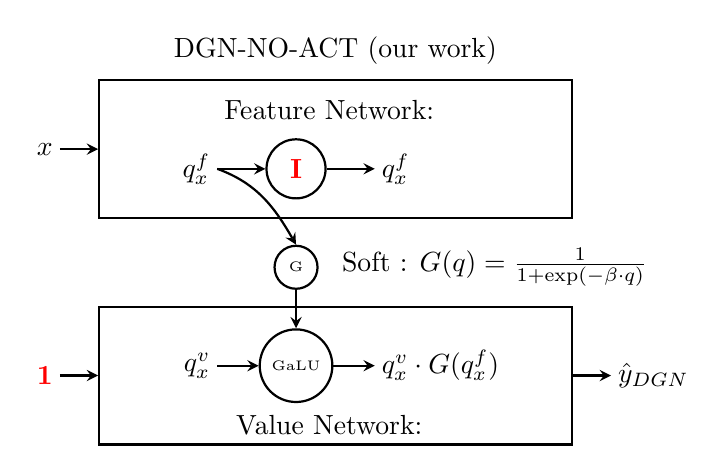
\begin{tikzpicture}
\node []  (fntext)at (3.5,1.5) {DGN-NO-ACT (our work)};
%Feature Network
\node [draw,
	minimum width=6cm,
	minimum height=1.75cm,
	thick
]  (fnbox)at (3.5,0.25) {};
\node []  (fntext)at (3.5,0.75) {Feature Network: $\Tf$};
%\node []  (fnnote)at (5.0,-0.5) {\tiny{\color{red}\textbf{No Non-Linear Activations}}};


%Feature Network Input
\node (fin) [left of=fnbox,node distance=3.5cm, coordinate] {};
\node[left=-1pt] at (fin.west){$x$};
\draw[-stealth, thick] (fin.center) -- (fnbox.west);

%Feature Network Output
%\node (fout) [right of=fnbox,node distance=3.5cm, coordinate] {};
%\node[right=-1pt] at (fout.west){$\hat{y}_{\text{f}}$};
%\draw[-stealth, thick]  (fnbox.east)--(fout.center);


%ReLU Circle
\node[draw,
	circle,
	minimum size=0.75cm,thick,
] (relu) at (3,0){{{\color{red}\textbf{I}}\mbox{}\mbox{}}};
%ReLU Input
\node (b) [left of=relu,node distance=1cm, coordinate] {};

\node[left=-1pt] at (b.center){$q^\text{f}_x$};
\draw[-stealth, thick] (b.east) -- (relu.west);


%ReLU Output
\node (c) [right of=relu,node distance=1cm, coordinate] {};
\node[right=-1pt] at (c.center){$q^\text{f}_x$};
\draw[-stealth, thick] (relu.east) -- (c.west);
	

%Value Network

\node [draw,
	minimum width=6cm,
	minimum height=1.75cm,
	thick
]  (vnbox)at (3.5,-2.625) {};

\node []  (vntext)at (3.5,-3.25) {Value Network: $\Tv$};
%\node []  (vnnote)at (5.25,-2) {\tiny{\color{red}\textbf{Input Only Via Gates}}};

%Value Network Input
\node (vin) [left of=vnbox,node distance=3.5cm, coordinate] {};
\node[left=-1pt] at (vin.west){{\color{red}$\mathbf{1}$}};
\draw[-stealth, thick] (vin.center) -- (vnbox.west);

%Value Network Output
\node (vout) [right of=vnbox,node distance=3.5cm, coordinate] {};
\node[right=-1pt] at (vout.west){$\hat{y}_{\text{DGN}}$};
\draw[-stealth, thick]  (vnbox.east)--(vout.center);


%Gating Circle
\node[draw,
	circle,
	minimum size=0.0625cm,thick,
] (gating) at (3,-1.25){\tiny{G}};
\node[right=6pt] at (3.25,-1.25){Soft : $G(q)=\frac{1}{1+\exp(-\beta\cdot q)}$};

%GaLU Circle
\node[draw,
	circle,
	minimum size=0.75cm,thick,
] (galu) at (3,-2.5){\tiny{GaLU}};

\draw [-stealth,thick]   (b) to[out=-20,in=120] (gating.north);
\draw [-stealth,thick]   (gating.south) -- (galu.north);



%GaLU Input
\node (d) [left of=galu,node distance=1cm, coordinate] {};
\node[left=-1pt] at (d.center){$q^\text{v}_x$};
\draw[-stealth, thick] (d.east) -- (galu.west);
%GaLU Output
\node (e) [right of=galu,node distance=1cm, coordinate] {};
\node[right=-1pt] at (e.center){$q^\text{v}_x\cdot G(q^\text{f}_x)$};
\draw[-stealth, thick] (galu.east) -- (e.west);
	
\end{tikzpicture}


}
\end{minipage}
\end{minipage}
\caption{DGN}
\label{fig:dgn}
\end{figure}

As mentioned in \Cref{sec:intro}, a deep gated network(DGN) setup is an alternative way to compute path-by-path, that is, the to compute the inner product of the neural path feature and neural path value. In this section, we first describe DGN in prior work \citep{npk}:  consitituent parts, information flow, purpose and training. We then discuss the two fundamental conceptual issues that make this DGN `black box'. We then present our modified \texttt{DGN-NO-ACT} with an intutitve explanation of how the conceptual issues are overcome and  why it is an entirely interpretatble white box model. These intuitive explanations will be justified in theory and experiments in \Cref{sec:main}.

\textbf{DGN (prior work).} Consider a DNN with ReLUs with weights $\Theta\in\R^{\dnet}$. The DGN \emph{corresponding} to this DNN (see the left diagram in \Cref{fig:dgn}) has two networks of \emph{identical archicture} (to the DNN) namely the feature network and value network with distinct weights $\Tf\in\R^{\dnet}$ and $\Tv\in\R^{\dnet}$ respectively. The main difference between the feature and value networks is in the activations. The feature network has ReLUs which turn `on/off' based on their pre-activation signal, and the value  network has gated linear units (GaLUs) \citep{sss,npk}. Each GaLU multiplies its pre-activation input by an external gating signal. Since the feature and value networks have identical architecture, there is an one-to-one correspondance between the ReLUs and GaLUs in the respective networks.
In the DGN, the external gating signal to the GaLU is derived from the pre-activation input of the corresponding ReLU. The feature network deals with the primal layer-by-layer computations, the pre-activations from the feature network generate the gates, which are then used to switch `on/off' the corresponding GaLUs in the value network: this realises $\phi_{\Tf}(x)$. The value network realises $v_{\Tv}$ and computes the output $\hat{y}_{\text{DGN}}(x)=\ip{\phi_{\Tf}(x),v_{\Tv}}$.

\textbf{DGN Training.} The primary use of the DGN was to measure the information in the gates of a DNN with ReLU. For this, the feature network (which is a DNN with ReLU) is \emph{pre-trained} with $\hat{y}_f$ as the output. Then the feature network is frozen and the value network is trained, i.e., in $\hat{y}_{\text{DGN}}(x)=\ip{\phi_{\Tf}(x),v_{\Tv}}$, $\phi_{\Tf}(x)$ is fixed and only $v_{\Tv}$ is learnt. Here, `hard'-gating is used: for pre-activation $q\in\R$, the gating value is $G(q) = \mathbbm{1}_{\{q>0\}}$. The secondary use of DGN is as an alternative/competetive model (for DNN) that learns  $\hat{y}_{\text{DGN}}(x)=\ip{\phi_{\Tf}(x),v_{\Tv}}$, by separately learning $\Tf$ and $\Tv$ starting from randomised initialisation.Here, `soft'-gating is used, where, $G(q)=\frac{1}{1+\exp({-\beta\cdot q})}$ ($\beta=10$ is a typical choice): this enables gradient to flow via the feature network. 
  
%$1.$ \textbf{Fixed Learnt (FL):} We \emph{pre-train} the feature network (which is a DNN with ReLUs), then \emph{freeze} the weights of the feature network, and then train the value network. This way we can measure information in the gates of a trained DNN.

%$2.$ \textbf{Fixed Random (FR):} We initialise the feature network at random, and then \emph{freeze} its weights and then train the value network. This way we can measure information in the gates of a DNN at initialisation. Here, the feature and value network can be either initialised with the same weights i.e., dependent initialisation (DI) or statistically independent weights  i.e., independent initialisation (II). 

%The secondary use of DGN is \textbf{decoupled learning} (DL) $\phi_{\Tf}(x)$ and $v_{\Tv}$ which is a comptetive proposal for DNN. For this, the gating is set to be `soft', $G(q)=\frac{1}{1+\exp({-\beta\cdot q})}$ (we used $\beta=10$ in our experiments). This allows the gradient to flow through the feature network. Here, $\Tf$ and $\Tv$ are initialiased statistically independent and then train both of them.

%To summarise the primal and secondary uses, one can say that the DGN operates in four modes namely FL, FR-II, FR-DI and DL.


\textbf{DGN-NO-ACT(our model)}(see right diagram in \Cref{fig:dgn}). We replace the ReLUs in the feature network with \emph{identity} maps, i.e., $I(q) = q$. Thus, in the \texttt{DGN-NO-ACT}, the transformation from input to the pre-activations is entirely linear and is amenable to interpertation via standard spectral analysis using linear algebraic tools. The pre-activations trigger the gates, which then dictates the path activity. The value network is given only given $\mathbf{1}$ as input and hence $v_{\Tv}\in \R^{\text{total\,paths}}$ is a vector that does not depend on the input, and $\phi_{\Tf}(x)\in(0,1)^{\text{total\,paths}}$ is a very simple feature vector. % and the output $\hat{y}_{\text{DGN}}(x)=\ip{\phi_{\Tf}(x),v_{\Tv}}=\sum_{p}\phi_\Tf(x,p)v_\Tv(p)$ is equal to \emph{\textbf{the summation of `path value' weighted by the `path activations'}}. 
Thus, the \texttt{DGN-NO-ACT} can be seen to disentangle the `primal linear' feature network which generates the gates, which in turn activate the paths in the value network which is the `dual linear'.

\textbf{Remark.} Presenting the value network with $\mathbf{1}$ is very counter intutive, which will get justfied in theory as well as experiments in the next section. As a quick check, we the test accuracies of a DNN $4$ with convolutional layers and global-average-pooling (GAP), its corresponding DGN and \texttt{DGN-NO-ACT} on CIFAR-10 are {\bf{DNN: $80.4\%$,  DNG: $79.4\%$, \texttt{DGN-NO-ACT} : $74.5\%$}}.



\begin{comment}
\begin{wrapfigure}{r}{0.2\textwidth}
\centering
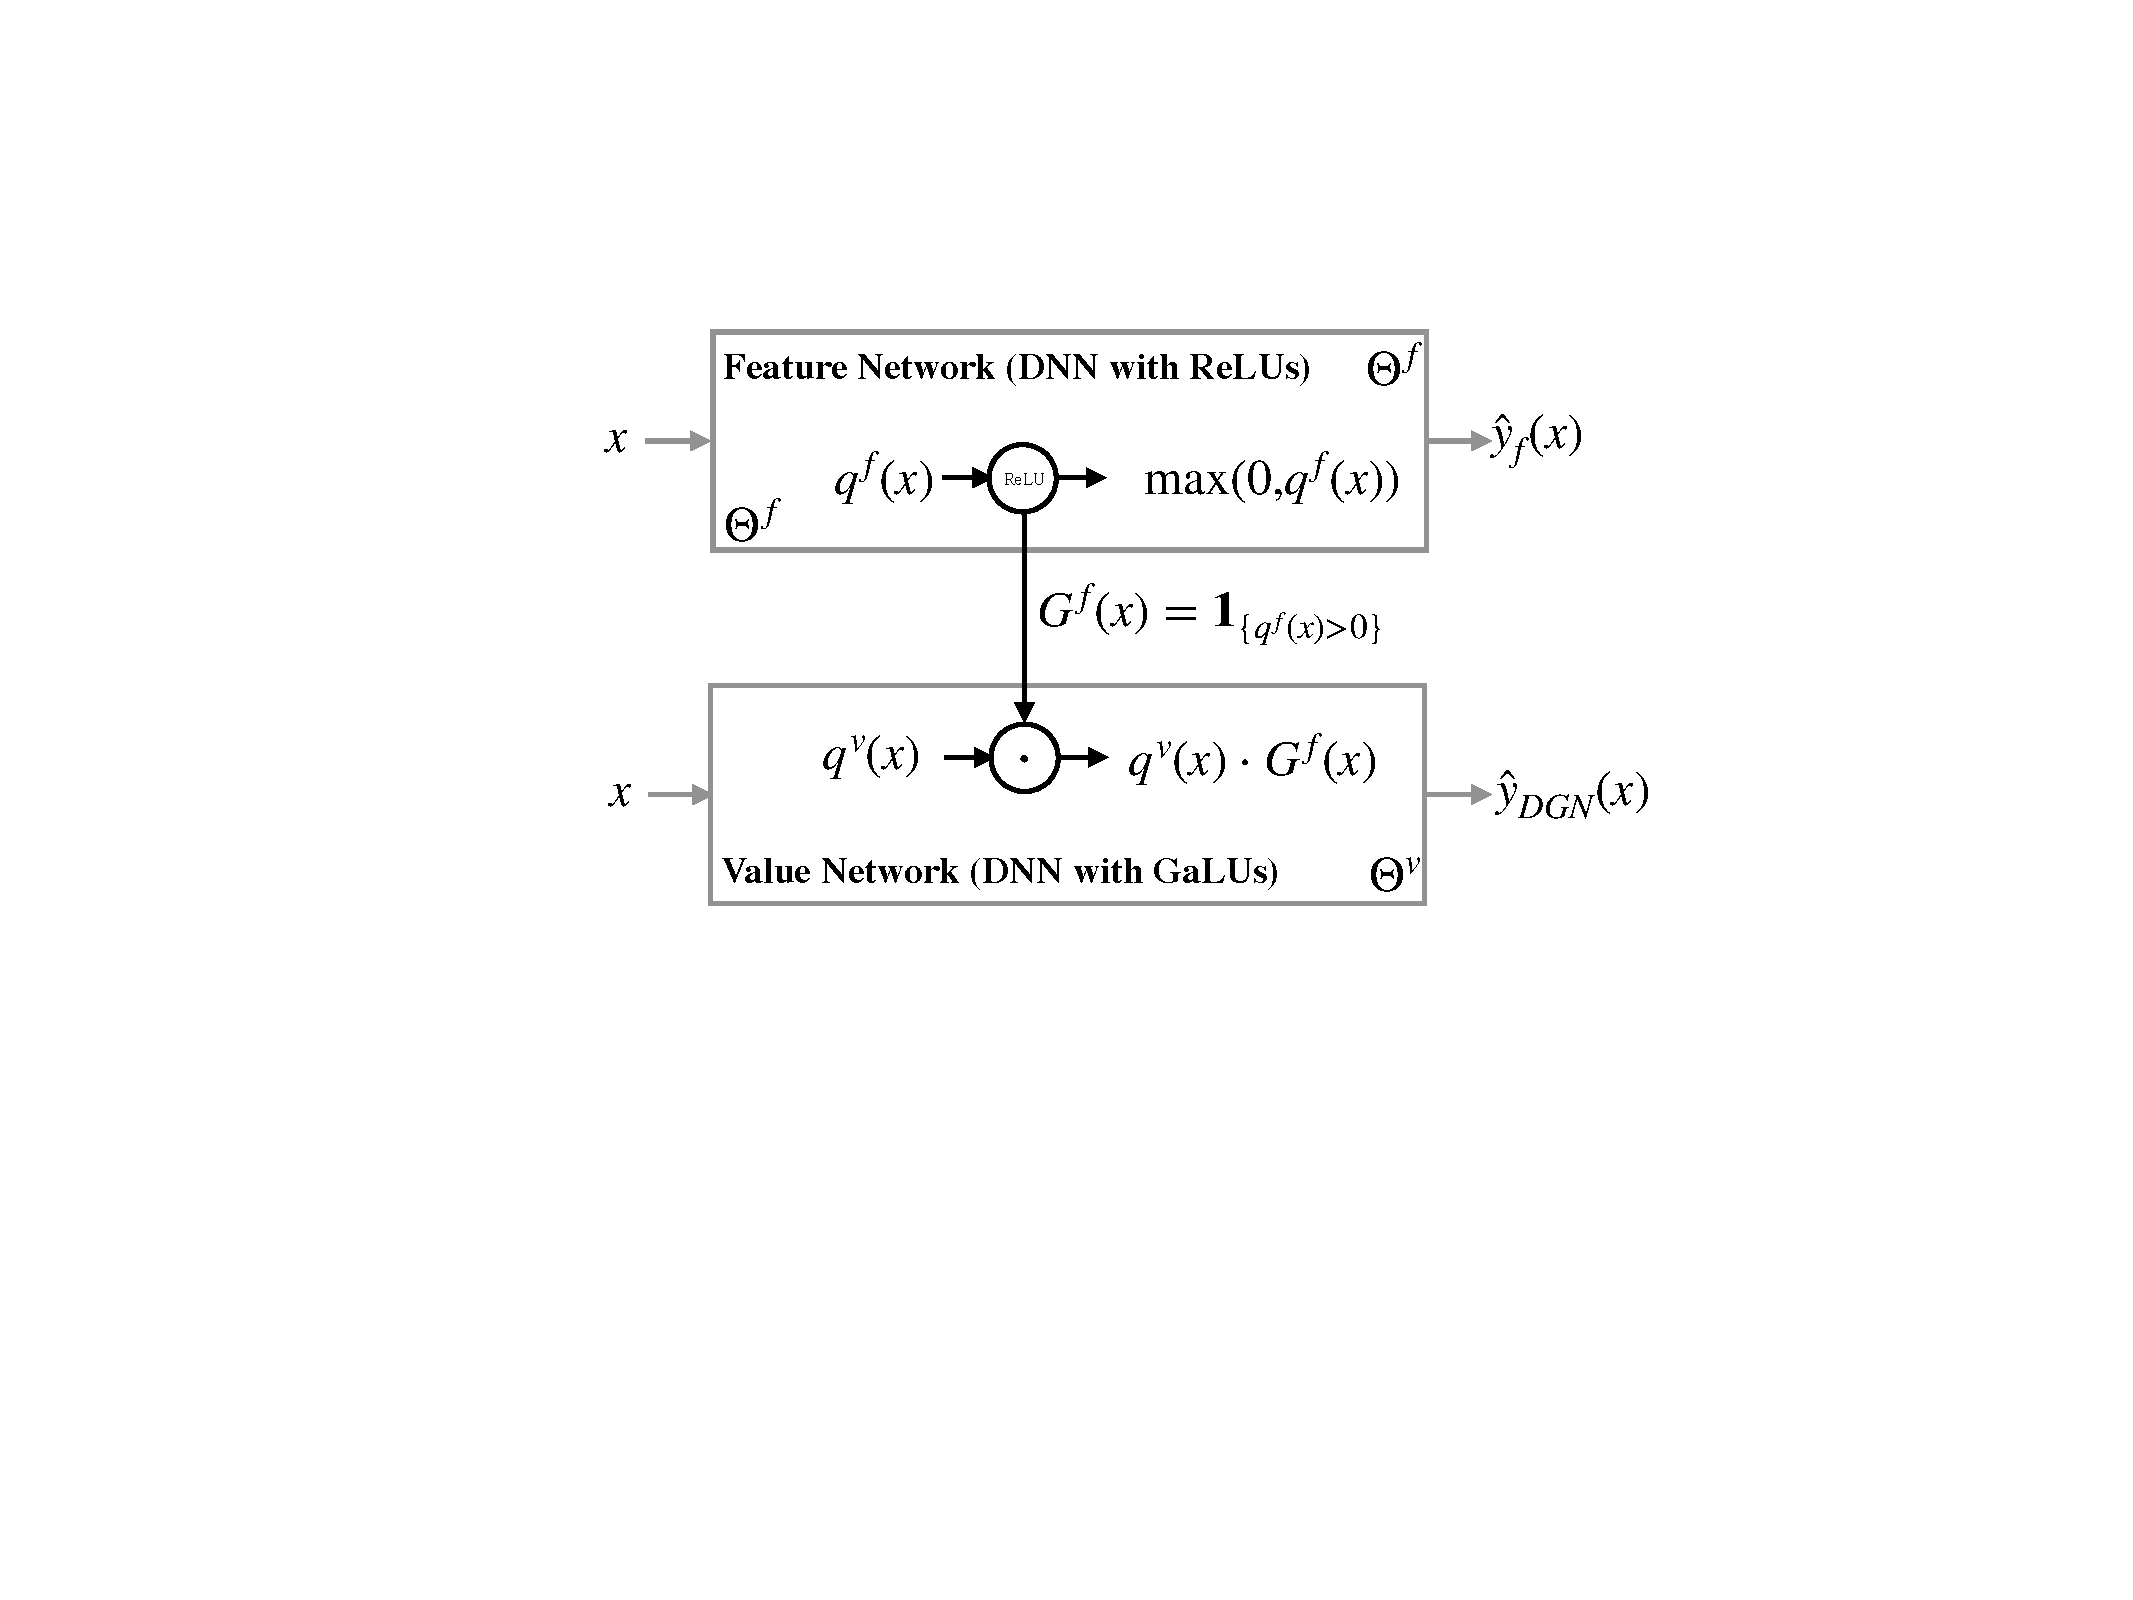
\includegraphics[scale=0.1]{figs/dgn-nips.pdf}
\caption{DGN}
\label{fig:dgn}
\end{wrapfigure}
\end{comment}

%Since $\hat{y}_{\Theta}(x)=\ip{\phi_{x,\Theta},v_{\Theta}}$, during training, as $\Theta$ is learnt, both the NPFs and NPV are also learnt. To understand their roles better, $\phi_{x,\Theta}$ and $v_{\Theta}$ have to be separated.  This is achieved by the deep gated network (DGN) setup (see \Cref{fig:dgn}), which has two networks of \emph{identical architecture} namely the \emph{feature network} ($\Tf\in\R^{d^{\text{f}}_{\text{net}}}$) which holds the NPFs (i.e., the gating information) and the \emph{value network} ($\Tv\in\R^{d^{\text{v}}_{\text{net}}}$) which holds the NPV.  The combined parameterisation is denoted by $\Theta^{\text{DGN}}=(\Tf,\Tv)\in \R^{d^{\text{f}}_{\text{net}}+d^{\text{v}}_{\text{net}}}$.  The feature network is a DNN with ReLUs and the value network is a DNN with \emph{Gated Linear Units (GaLUs)} (terminology used in [\citenum{sss}]) whose output is the product of its pre-activation input $q^{\text{v}}(x)$and the external gating signal $G^{\text{f}}(x)$ (see \Cref{fig:dgn}). In \Cref{fig:dgn}, the main output of the DGN is $\hat{y}_{\text{DGN}}(x)$, while the other output $\hat{y}_{\text{f}}(x)$ is used to \emph{pre-train} the gates (see \Cref{sec:exp}).

